\section{Le conte, vecteur de transmission d'humanisme en déclin}

\begin{figure}[h!]
    \centering
    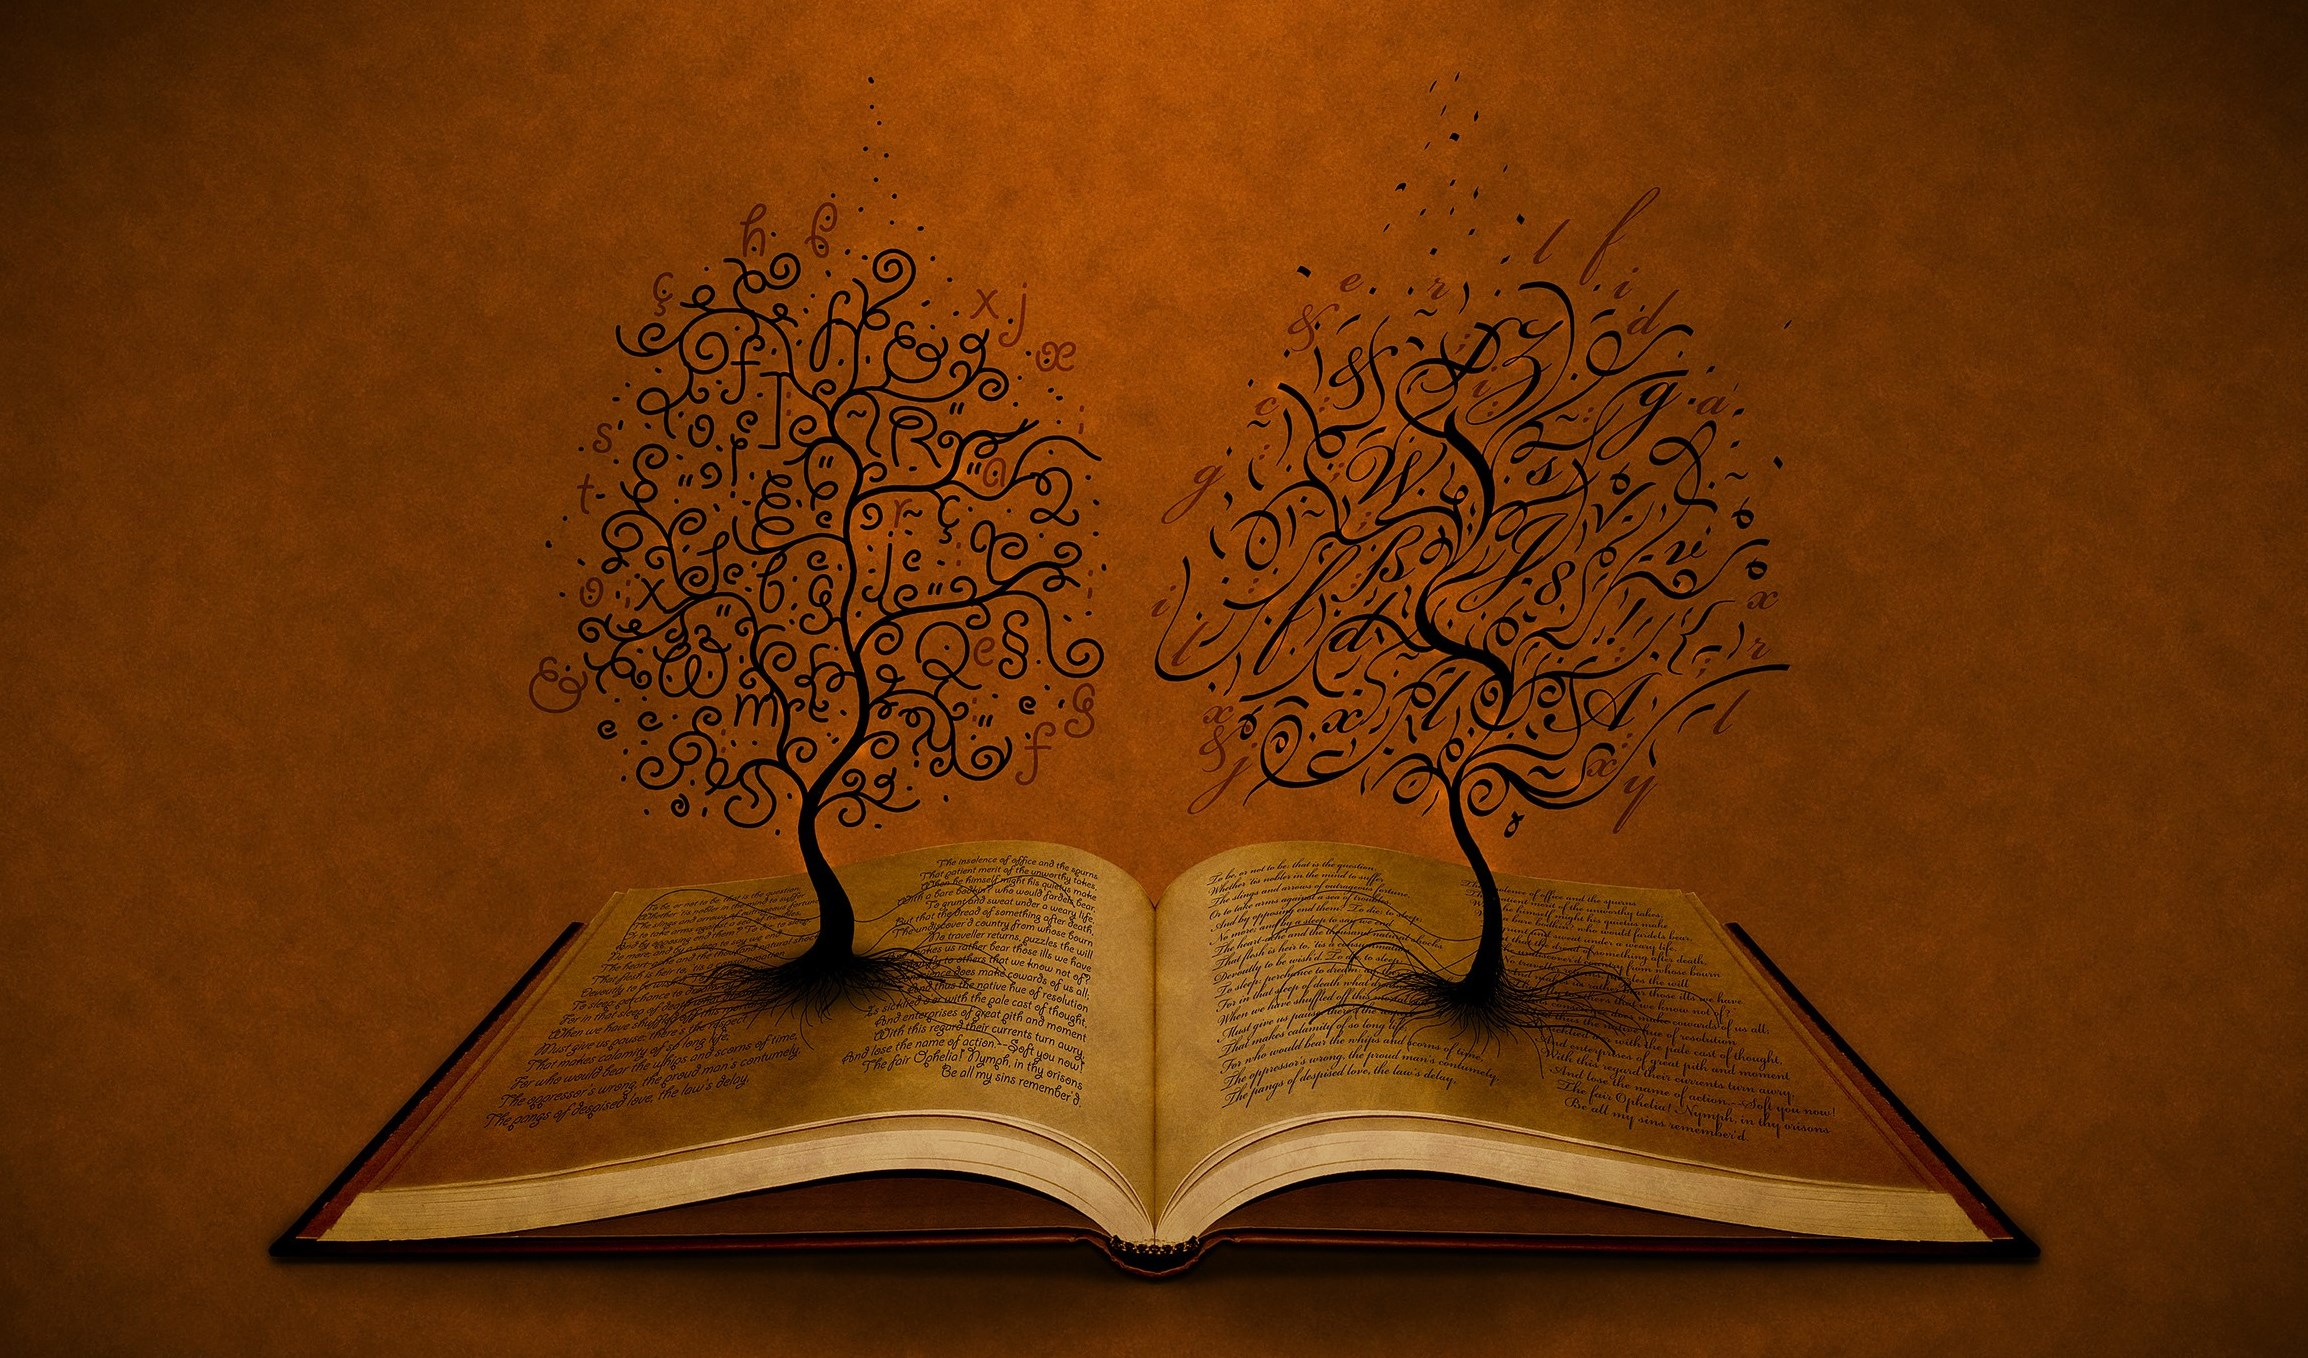
\includegraphics[width=0.80\linewidth]{img/tale_book.jpg}
    \caption{Vue d'artiste d'un livre de conte}
\end{figure}

\subsection{Vecteur d'expérience}
\begin{shadequote}
Le premier véritable récit est et demeure le conte. \par\emph{Walter Benjamin, Der Erzähler}
\end{shadequote}

Dans ses origines, lesquelles se perdent dans l'histoire de l'humanité, et encore aujourd'hui, le conte oral est considéré comme un vecteur destiné à perpétuer l'expérience d'un vécu et renouveler la tradition portée par ses conteurs. Ces contes, que l'on peut associer à une littérature orale où le conteur endosserait un rôle de narrateur, s'opposent originellement aux mythes car voués à « rapporter à quelqu'un un fait réel »\cite{cnrtl}.\\

On notera alors deux figures emblématiques du conteur ; d'une part un personnage sédentaire, d'autre part un voyageur. Le premier perpétue un « lointain temporel »\cite{nouss2003conteur}, c'est-à-dire une histoire riche d'expériences passées et transmise à travers les générations. On associera donc naturellement ces êtres à la mémoire d'un peuple, gardiens de la tradition et du savoir des générations passées. Le second parcourt ce monde à la recherche de rencontres humaines et d'échanges culturels, ce dans le but de diffuser à tout un chacun un « lointain spatial » \textit{(ibid)}, récits d'expériences vécues ou entendues en d'autres lieux.\\

Le métier de conteur revêt donc une dimension sociale d'importance, associée à la transmission systématique d'une expérience qui est la teneur principale du conte. Une interprétation probable de la cause d'une perte de vitesse manifeste de la transmission orale via le conte résiderait alors dans la valeur accordée au conte par son public. En effet, l'intérêt porté par les jeunes générations à l'expérience serait en net déclin, notamment de par l'omniprésence de l'information journalistique à travers une multitude de médias. Cette information rapportée notifiant son public captif des derniers évènements survenus, analysés et expliqués, elle s'oppose magistralement au conte, ce dernier laissant à son auditoire le soin d'une réflexion visant à une interprétation propre accompagnée de ses conclusion. Le conte délivre en effet un fait nu, valorisant le processus intellectuel de son public.\\

La valeur des contes ne résiderait donc pas dans leur intrigue, mais dans la mise en valeur de l'acte qu'est le vécu d'une expérience. Les contes véhiculent ainsi une conception de l'être humain et de la vie, celle de vivre des expériences, de traverser des épreuves, et de les surmonter.

On notera enfin une dérive du genre à travers l'époque contemporaine, les récits véhiculés ne faisant plus nécessairement référence à un vécu réel, mais plus souvent « brodé » ou façonné, néanmoins souvent porteur d'une morale visant à enrichir son auditoire.\\

\begin{figure}[h!]
    \centering
    
\includegraphics[width=0.80\linewidth]{img/storyteller.png}
    \caption{Le conte, vecteur de transmission de la tradition}
\end{figure}

\clearpage


\subsection{Un processus d'attention flottante}

\begin{shadequote}
[...] en conformant son choix à son expectative, on court le risque de ne trouver que ce que l'on savait d'avance.
\par\emph{Sigmund Freud, Ratschl{\"a}ge f{\"u}r den Arzt bei der psychoanalytischen Behandlung}
\end{shadequote}

Focalisé sur l'écoute du conte transmis, l'auditoire serait par ailleurs l'objet du procédé « d'attention flottante »\cite{freud1996ratschlage}. Cet état d'esprit, découvert par Freud, consisterait en l'absence d'attention dirigée ou focalisée, ce dans le but de permettre à l'auditeur de s'oublier lui-même afin que « les mots qu'il entend[e] s'inscrivent profondément en lui » \cite{benjamin1991gesammelte}.\\

Cette situation est notamment recommandée aux psychanalystes, lesquels se doivent de ne pas laisser leurs préjugés influencer leur diagnostique. Afin de percevoir pleinement l'inconscient du patient, il est en effet conseillé à ces praticiens de modérer leur hâte d'interprétation et d'éviter l'exercice d'une attention maintenue, laquelle ne saurait durer et aurait pour effet de ne sélectionner comme importants qu'une partie des éléments fournis. L'écoute « flottante », définie par une attention non soutenue et égale apportée à ce qui est entendu, favoriserait alors la libre association des idées et la conservation mémorielle de l'ensemble des détails en apparence insignifiants dont les corrélations ne se feront qu'ultérieurement.\\

Détendu et vivant pleinement le récit qui lui est narré, le public ferait donc l'expérience de ce procédé, lequel lui permettrait une mémorisation et assimilation certaine. C'est une fois la séance terminée, sur le chemin du logis ou une fois endormi, que le processus de réflexion inconsciente du public décèlerait les subtilités et le message profond présent dans l'histoire racontée. La transmission orale se prêterait donc naturellement à l'assimilation d'une morale, de même qu'à l'évolution de l'être par l'acquisition du vécu transmis.


\subsection{De l'autorité mortuaire}

\begin{shadequote}
Le parfait récit naît de l'accumulation de ses versions successives. \par\emph{Walter Benjamin, Der Erzähler}
\end{shadequote}

Selon Walter Benjamin, le conteur tiendrait de la mort son autorité. En effet, un conte étant constitué de vécu, une vie chargée d'expériences fondera une sagesse et un savoir dont la transmission n'en sera que plus riche ; « La mort est la sanction de tout ce que relate le conteur » \textit{(ibid)}. À l'heure de sa mort, toute personne devient donc digne d'être écoutée.

Il faut en outre prendre en compte dans le cas d'un récits perpétué, que chaque conteur apose sa marque à celui-ci, le transformant subtilement de par son vécu. Tout conte transmis n'en est donc que plus riche.\\


Revenant au déclin des contes dans notre société, il est devient à présent crucial d'étudier l'évolution de la conception de la mort par l'humain comme cause potentielle de celui-ci.

Une étude du siècle dernier révèle en effet un bouleversement certain de la conception sociale de la mort dans nos moeurs. Riche en progrès technologiques et en morts médiatisées, celui-ci s'est accompagné d'une acceptation de la mort en masse (Hiroshima), chargée de souffrance (camps de déportation durant la seconde guerre mondiale), banalisée et quotidienne (films et journaux télévisés).

La conception mortuaire du public ayant évoluée, l'autorité que le conteur en retire en est de ce fait impactée. Puisque la mort d'un être humain ne revêt plus alors autant d'importance, il en va de même pour celle de son vécu, et de ses contes. Rappelons ici que l'existence d'un conte réside dans la mémoire de son auditoire, et sa survie dans la transmission de celui-ci par ses conteurs. Puisqu'un conte meurt s'il n'est pas transmis, nombreux sont aujourd'hui les récits délaissés, oubliés, puis enterrés.\\

De par l'évolution de la conception mortuaire et de l'intérêt porté à l'expérience, le déclin du conte et des traditions ne peuvent aujourd'hui qu'être constatés. Cette époque observe néanmoins un attrait grandissant envers une pratique sociale, ludique voire théâtrale : le jeu de rôle.

\clearpage
